% ============================================================
%  Modul 5 — Sistem Build dengan GCC
% ============================================================

\chapter{Sistem Build dengan GCC}
\label{chap:modul-05}

% --- 1. Tujuan dan Output Praktikum ---
\section{Tujuan dan Output Praktikum}

\subsection{Tujuan Praktikum}
Setelah menyelesaikan praktikum ini, mahasiswa diharapkan mampu:
\begin{enumerate}
	\item Memahami proses kompilasi kode sumber C/C++ menggunakan \textit{GNU Compiler Collection} (GCC).
	\item Mengenal dan mempraktikkan tahapan dalam proses \textit{build}: preparasi, kompilasi, perakitan (\textit{assembly}), dan \textit{linking}.
\end{enumerate}

\subsection{Output Praktikum}
Pada akhir praktikum ini, mahasiswa diharapkan menghasilkan:
\begin{itemize}
	\item File kode sumber C sederhana yang berhasil dikompilasi menjadi \textit{executable}.
	\item Hasil dari setiap tahapan proses kompilasi (\texttt{.i}, \texttt{.s}, \texttt{.o}).
\end{itemize}

% --- 2. Dasar Teori ---
\newpage
\section{Dasar Teori}

\subsection{GNU Compiler Collection (GCC)}
GCC awalnya merupakan \textit{GNU C Compiler}, namun kini telah berkembang mendukung berbagai bahasa pemrograman seperti C, C++, Objective-C, Fortran, Ada, Go, dan D \cite{gough2004introduction}. GCC adalah standar kompiler yang banyak digunakan dalam sistem operasi mirip UNIX (Unix-like), terutama distribusi Linux. GCC dirancang agar kuat, fleksibel, teroptimasi, dan mendukung banyak arsitektur perangkat keras.

\subsection{Tahapan Kompilasi GCC}
Proses mengubah (\textit{build}) suatu kode sumber bahasa tingkat tinggi (seperti C) menjadi program (\textit{executable}) yang bisa dijalankan komputer dilakukan melalui 4 proses sekuensial \cite{bryant2015computer}:

\subsubsection{Preprocessing (Pra-kompilasi)}
Pada tahap ini, kompiler menginisialisasi pengerjaan arahan preprosesor (seperti \texttt{\#include}, \texttt{\#define}). Ia menambahkan kode dari \textit{header file}, mengganti makro, dan membuang komentar pada kode sumber awal (misal \texttt{main.c}). Tahapan ini mendayagunakan perangkat lunak \textit{C Preprocessor} (\texttt{cpp}) dan menghasilkan file berekstensi \texttt{.i}.

\subsubsection{Compilation (Kompilasi)}
Tahap ini mengambil keluaran dari preprosesor (\texttt{.i}) lalu menerjemahkannya ke dalam kode bahasa rakitan (\textit{assembly language}) spesifik sesuai arsitektur mesin tujuan. Hasil dari tahap kompilasi ini adalah sebuah teks instruksi assembli berekstensi \texttt{.s}.

\subsubsection{Assembly (Perakitan)}
Kode \textit{assembly} (\texttt{.s}) diproses ke dalam bahasa mesin (\textit{machine level language} berformat biner) yang dapat dimengerti sistem komputer. Perangkat lunak yang merangkap proses ini disebut \textit{Assembler} (\texttt{as}). Output dari tahapan ini adalah file objek (\textit{object file}) berekstensi \texttt{.o}. File ini masih belum bisa dieksekusi sebelum dihubungkan dengan library atau file objek lain.

\subsubsection{Linking (Penautan)}
Fase terakhir merupakan tahap penggabungan di mana berbagai file objek pendukung (\texttt{.o}) disatukan menjadi satu program utuh beserta file pustaka bawaan (\textit{library file}). Contoh umum adalah penautan dengan glibc (standar pustaka C). Jika menggunakan pustaka pihak ketiga semisal \textit{math} atau \textit{pthread}, tautannya juga dideklarasikan di sini (\texttt{-lm}, \texttt{-lpthread}). Perangkat lunaknya dinamai \textit{Linker} (\texttt{ld}). Outputnya adalah file \textit{executable}.

Tabel \ref{tab:m05-dasar-teori} merangkum hal-hal penting terkait flag GCC yang sering digunakan.

\begin{table}[h]
	\caption{Ringkasan Flag GCC Umum}
	\label{tab:m05-dasar-teori}
	\centering
	\begin{tabulary}{\textwidth}{|L|L|}
		\hline
		\textbf{Flag} & \textbf{Penjelasan Singkat} \\ \hline
		\texttt{-o}     & Spesifikasikan nama file output \\ \hline
		\texttt{-Wall}  & Nyalakan peringatan kompilator ("Wall" = Warning all) \\ \hline
		\texttt{-E}     & Berhenti setelah tahap Preprocessing tanpa melakukan yang lain \\ \hline
		\texttt{-S}     & Hasilkan file .s, jangan assemble (berhenti di tahap Compilation) \\ \hline
		\texttt{-c}     & Menghasilkan file output berbentuk assembli murni atau .o (berhenti di tahap Assembly) \\ \hline
		\texttt{-g}     & Sertakan informasi \textit{debugging} (berguna menggunakan GDB) \\ \hline
	\end{tabulary}
\end{table}

% --- 3. Alat dan Bahan ---
\newpage
\section{Alat dan Bahan}
\label{sec:m05-alat-bahan}

\subsection{Perangkat Keras}
\begin{itemize}
	\item PC/Laptop dengan arsitektur prosesor x86\_64 atau lainnya.
	\item Ruang penyimpanan yang cukup untuk menyimpan hasil \textit{build}.
\end{itemize}

\subsection{Perangkat Lunak}
\begin{itemize}
	\item Sistem Operasi berbasis Linux (Ubuntu Desktop/Server) atau WSL 2.
	\item Instalasi \textit{build-essential} (mencakup \texttt{gcc}, \texttt{make}, dan lainnya).
	\item Kode editor (seperti Vim, Nano, atau VS Code).
\end{itemize}

% --- 4. Langkah-Langkah Praktikum ---
\newpage
\section{Langkah-Langkah Praktikum}

\subsection{Persiapan Lingkungan}
\label{sec:m05-persiapan}
Sebelum memulai kompilasi, pastikan lingkungan memadai dan gcc sudah diatur dengan benar di dalam sistem Anda.

Berikut adalah tahapan-tahapan yang harus Anda selesaikan secara berurutan:

\begin{enumerate}
	\item Buka terminal (atau distro WSL yang telah Anda konfigurasikan).
	\item Pastikan instrumen penunjang sudah ter-install dengan paket yang disarankan (\textit{build-essential}).
	      \begin{lstlisting}[language=bash, caption={Perintah verifikasi lingkungan}]
sudo apt update
sudo apt install build-essential -y
gcc --version
make --version
    \end{lstlisting}

	      \begin{figure}[htbp]
		      \centering
		      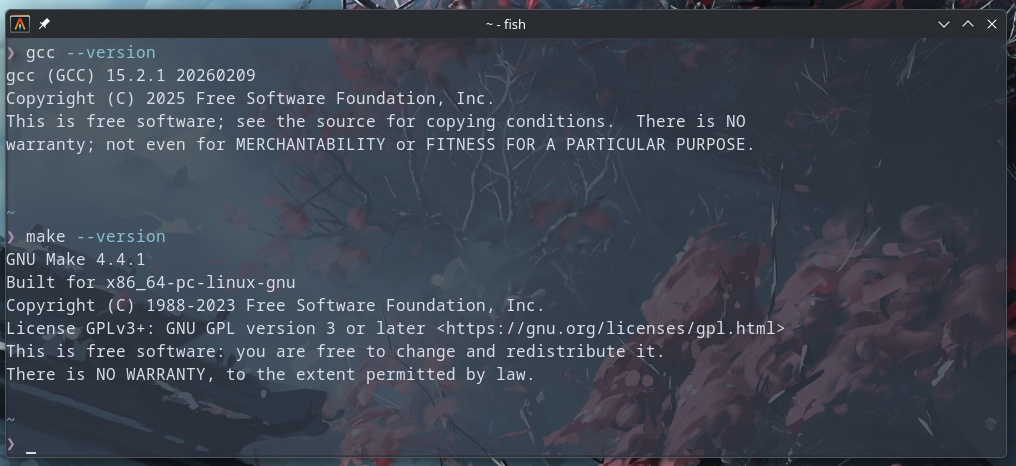
\includegraphics[width=0.75\textwidth]{Figure/05/gcc-make.png}
		      \caption{Verifikasi Versi GCC dan Make}
		      \label{fig:m05-gcc-make}
	      \end{figure}

	\item Buat sebuah direktori bernama \texttt{praktikum-gcc} untuk praktikum modul ini.
	      \begin{lstlisting}[language=bash, caption={Membuat direktori kerja}]
mkdir praktikum-gcc
cd praktikum-gcc
    \end{lstlisting}
\end{enumerate}

\subsection{Sesi 1: Siklus Hidup Kompilasi C}
\label{sec:m05-sesi-1}
Kita akan membongkar proses kompilasi penuh sebuah program C sederhana menggunakan sekumpulan \textit{flags} untuk menangguhkan setiap tahapan \textit{build}, sehingga Anda dapat memahaminya secara parsial.

Berikut adalah tahapan-tahapan yang harus Anda selesaikan secara berurutan:

\begin{enumerate}
	\item Buatlah sebuah file kode sumber C bernama \texttt{salam.c} menggunakan teks editor terminal \texttt{nano}:
	      \begin{lstlisting}[language=bash, caption={Membuat file dengan nano}]
nano salam.c
    \end{lstlisting}

	\item Di dalam \texttt{nano}, ketik atau salin kode bahasa C berikut:
	      \begin{lstlisting}[language=c, caption={Isi salam.c}]
#include <stdio.h>
#define PESAN "Halo, Selamat datang di Pembelajaran Sistem Operasi!"

int main() {
    printf("%s\n", PESAN);
    return 0;
}
    \end{lstlisting}
	      \textit{Simpan file di nano dengan menekan Ctrl+O, lalu Enter. Kemudian keluar dengan Ctrl+X.}

	      \begin{figure}[H]
		      \centering
		      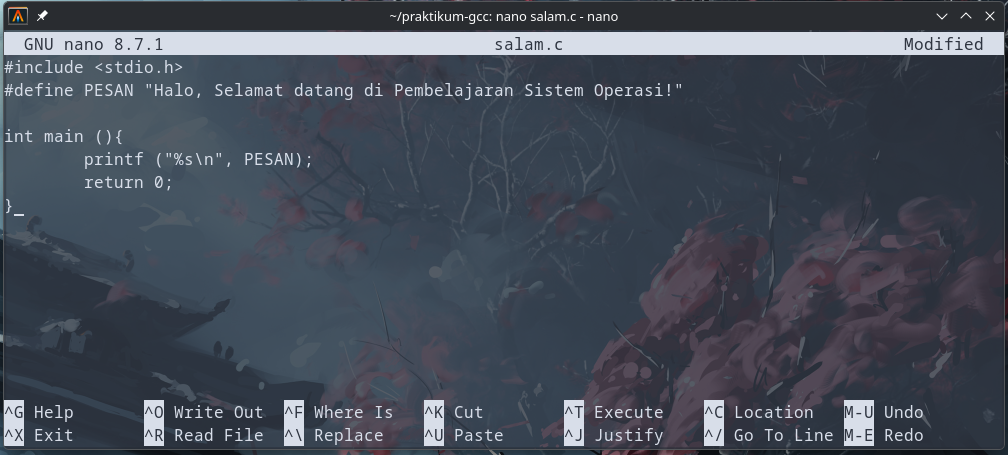
\includegraphics[width=0.75\textwidth]{Figure/05/nano-salam-c.png}
		      \caption{Membuat file salam.c dengan Nano}
		      \label{fig:m05-nano-salam-c}
	      \end{figure}

	\item Praktikkan tahapan pertama, yaitu \textbf{Preprocessing} (menginisialisasi header dan macro) secara manual dengan argumen (\texttt{-E}):
	      \begin{lstlisting}[language=bash, caption={Preprocessing}]
gcc -E salam.c -o salam.i
    \end{lstlisting}
	      Anda bisa melihat isi dari file hasil prakompilasi dengan \texttt{cat salam.i} atau \texttt{less salam.i}. Gulir ke bawah (atau tekan spasi di `less`), akan tampak baris macro `PESAN` telah diubah dengan nilai aslinya.

	      \begin{figure}[H]
		      \centering
		      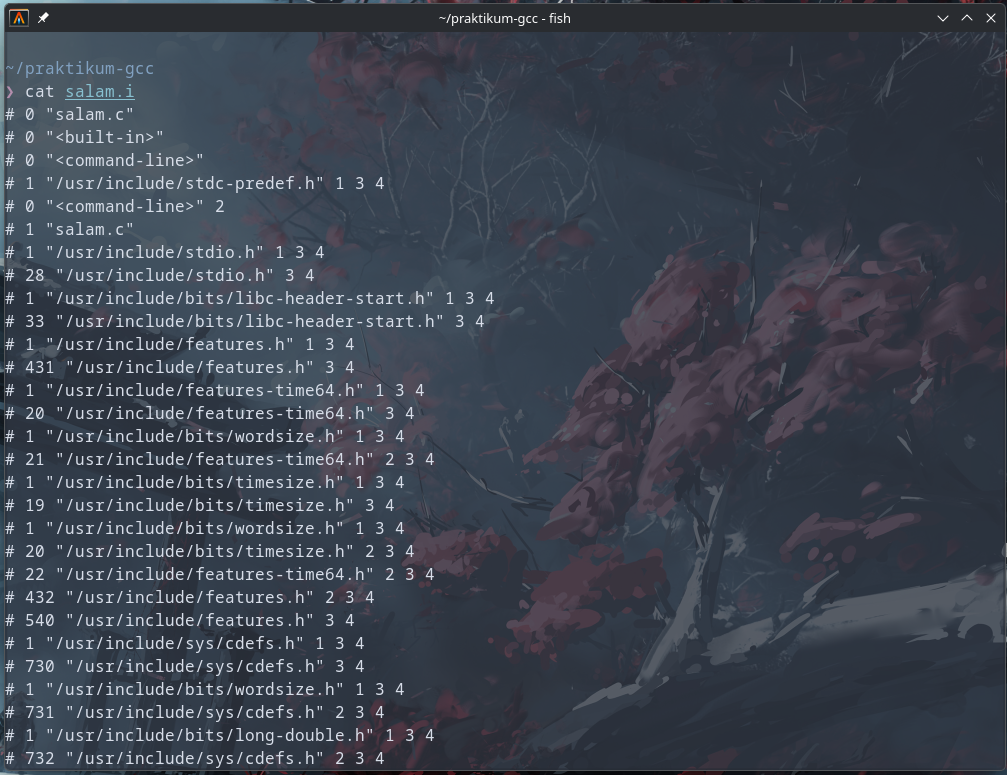
\includegraphics[width=0.75\textwidth]{Figure/05/salam-i.png}
		      \caption{Hasil Preprocessing}
		      \label{fig:m05-salam-i}
	      \end{figure}

	\item Praktikkan tahapan \textbf{Compilation} yang mengubahnya menjadi bahasa mesin/assembly (\texttt{-S}):
	      \begin{lstlisting}[language=bash, caption={Kompilasi menjadi Assembly}]
gcc -S salam.c -o salam.s
cat salam.s
    \end{lstlisting}
	      Teks output `cat` akan memunculkan instruksi-instruksi CPU yang rumit. Inilah yang disebut \textbf{assembly}.

	      \begin{figure}[H]
		      \centering
		      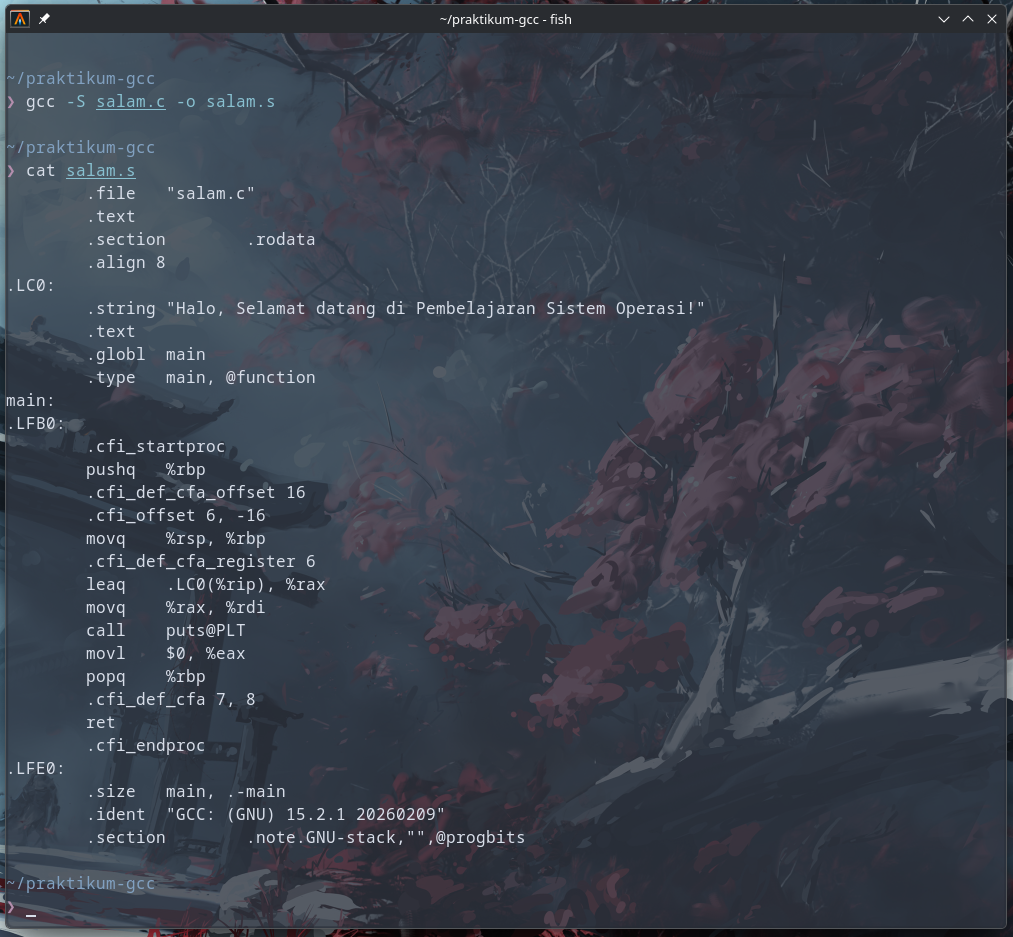
\includegraphics[width=0.75\textwidth]{Figure/05/salam-s.png}
		      \caption{Hasil Compilation}
		      \label{fig:m05-salam-s}
	      \end{figure}

	\item Praktikkan tahapan \textbf{Assembly} untuk merakitnya menjadi \textit{object file} biner (\texttt{-c}):
	      \begin{lstlisting}[language=bash, caption={Assemble menjadi file objek}]
gcc -c salam.c -o salam.o
    \end{lstlisting}
	      \textit{object file}  (\texttt{.o}) ini bukan lagi sebuah teks ASCII yang bisa dibaca manusia, ini adalah sebuah format instruksi mesin dalam bentuk biner. Anda tidak perlu membacanya dengan `cat`.

	      \begin{figure}[H]
		      \centering
		      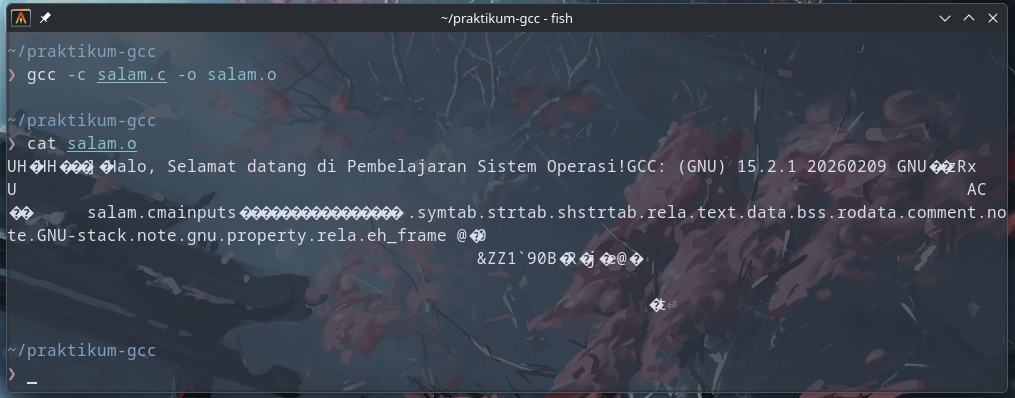
\includegraphics[width=0.75\textwidth]{Figure/05/salam-o.png}
		      \caption{Hasil Assembly}
		      \label{fig:m05-salam-o}
	      \end{figure}

	\item Tahap akhir, praktikkan \textbf{Linking} sebagai jembatan yang menyatukan semua kode objek dengan file pustaka internal menjadi file yang siap jalan (\texttt{Executable}):
	      \begin{lstlisting}[language=bash, caption={Linking menjadi Executable}]
gcc salam.o -o program_salam
    \end{lstlisting}

	\item Sekarang Anda bisa langsung mencoba menjalankan (run) file executablenya:
	      \begin{lstlisting}[language=bash, caption={Eksekusi program}]
./program_salam
    \end{lstlisting}
	      Hasilnya akan menampilkan pesan `Halo, Selamat datang di Pembelajaran Sistem Operasi!` di terminal.

	      \begin{figure}[H]
		      \centering
		      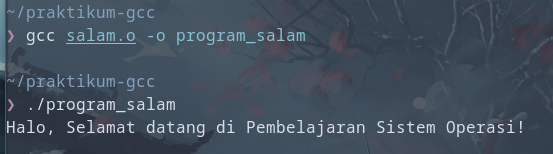
\includegraphics[width=0.75\textwidth]{Figure/05/program-salam.png}
		      \caption{Hasil Eksekusi Program Salam}
		      \label{fig:m05-program-salam}
	      \end{figure}
\end{enumerate}